\documentclass[a4paper]{report}
\usepackage[utf8]{inputenc}
\usepackage{hyperref}
\usepackage{a4wide}
\hypersetup{pdftitle={Dotprod},
pdfauthor={João Teixeira, José Ferreira},
colorlinks=true,
urlcolor=blue,
linkcolor=black}
\usepackage{subcaption}
\usepackage[cache=false]{minted}
\usepackage{listings}
\usepackage{booktabs}
\usepackage{multirow}
\usepackage{appendix}
\usepackage{tikz}
\usepackage{authblk}
\usepackage{bashful}
\usepackage{verbatim}
\usepackage{amssymb}
\usepackage{multirow}
\usepackage{mwe}
\usepackage[parfill]{parskip}
\usetikzlibrary{positioning,automata,decorations.markings}
\AfterEndEnvironment{figure}{\noindent\ignorespaces}
\AfterEndEnvironment{table}{\noindent\ignorespaces}

\usepackage{titlesec}

\titleformat{\chapter}[display]
   {\normalfont\large\bfseries}{\chaptertitlename\ \thechapter}{0pt}{\huge}
\titlespacing*{\chapter}{0pt}{0pt}{0pt}

\begin{document}

\title{Advanced Architectures\\Dotprod Implementations and Benchmarking}
\author{João Teixeira (A85504) \and José Filipe Ferreira (A83683)}
\date{\today}

\begin{center}
    \begin{minipage}{0.75\linewidth}
        \centering
        
\includegraphics[width=0.4\textwidth]{images/eng.jpeg}\par\vspace{1cm}
        \vspace{1.5cm}
        \href{https://www.uminho.pt/PT}
        {\color{black}{\scshape\LARGE Universidade do Minho}} \par
        \vspace{1cm}
        \href{https://www.di.uminho.pt/}
        {\color{black}{\scshape\Large Departamento de Informática}} \par
        \vspace{1.5cm}
        \maketitle
    \end{minipage}
\end{center}

\begin{abstract}
    \begin{center}
        This paper documents the development and benchmarking of different
        dotprod algorithms with the aim of analyzing, among others, the impact
        of matrix transposing, vectorization, paralllization and CUDA on the
        computation time
    \end{center}
\end{abstract}

\tableofcontents

\listoftables

\listoffigures

\chapter{Introduction}
In the last decades the hardware market has seen a shift towards the mass
availability of multicore CPUs and the constant increase of the computing power
of the GPUs. Due to this increased availability there is a growing need for
performance engineers and programmers capable of exploring this constantly
expanding field.

In this paper we will document the development and benchmarking of different
dotprod algorithms in order to study the impact of several alterations on the
basic dotprod implementation.

Firstly we will compare different sequential versions of the algorithm. Then we
will introduce blocking to the algorithm and vectorize it. Finally, to compare
the maximum performance of the CPU with the maximum performance of the GPU, a
parallelized version of the algorithm will be developed with OpenMP and a GPU
version will be developed making use of the CUDA API.

\chapter{Characterization of the hardware}
Our team's main laptop is a Lenovo ThinkPad X260. It is powered by a i5-6300U, a
dual-core hyperthreaded skylake cpu.

To get more information related to the CPU's memory hierarchy we used the
command \textit{lstopo} that displays a graphic with information related with
the cache size.
\begin{figure}[H]
    \centering
        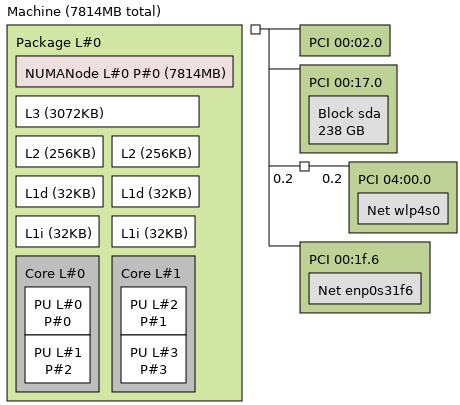
\includegraphics[width=0.5\textwidth]{images/lstopo.png}
        \caption{lstopo graphic}
\end{figure}

As it is visible in the picture above the CPU has 32KiB of L1 cache per core,
256KiB of L2 cache per core and 3072MiB L3 cache. It also has 7814MiB of Random
Access Memory(RAM) with minimum latency of 13.750 nano seconds acording to
vendor specs.

The computer used for obtaining the results during this paper was the node 662
of the search cluster at Universidade do
Minho\footnote[1]{\url{http://search6.di.uminho.pt}}. It is equipped with
a
dual Intel Xeon E5-2695v2 processor
with 24 cores and Nvidia Kepler K20m accelerators. This CPUs have 32 KiB of L1
cache for each core, 256KiB of L2 cache, 30MiB of L3 cache and 64GiB of RAM.

\chapter{Dotprod Implementation}
The dotprod is a mathematical operation between two matrices (A and B) that
results in another matrix (C). To obtain the position (i,j) in the matrix C we
need to multiply each value of the line i in the matrix A with each value of the
column j of the matrix B and add them.

When programming this behaviour it is commonly used a nested triple for loop
going from 0 to the size of the matrix. Each loop having a different variable
usually i, j and k. The variable i indexes the lines on the A matrix, the j
indexes the columns on the B matrix and the k is the loop that iterates over the
line and column.

\begin{figure}[H]
    \centering
        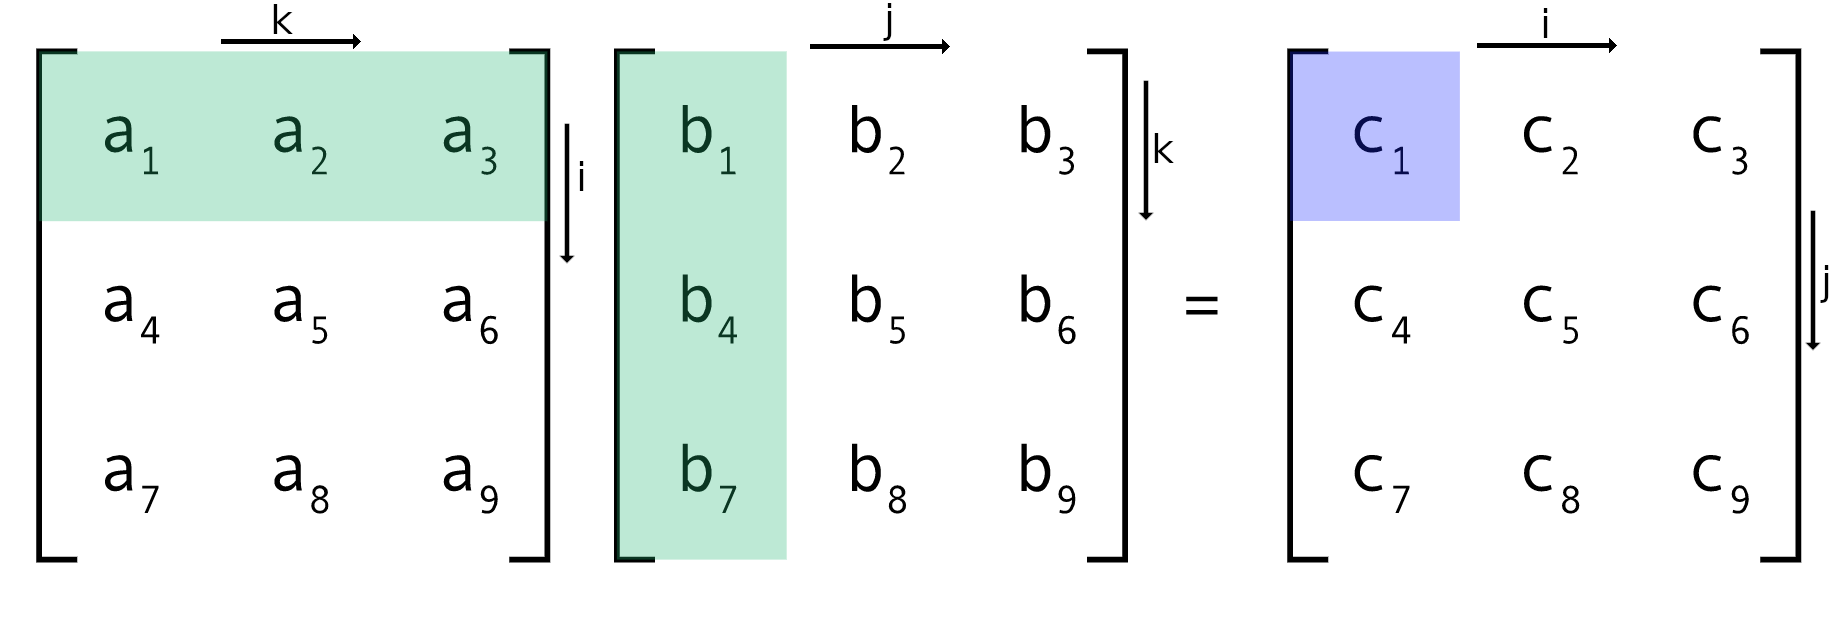
\includegraphics[width=0.7\textwidth]{images/matrix_mult.png}
        \caption{Dotprod Diagram}
\end{figure}

The first implementation of the algoritm had the nested loop in the order
\textbf{i-j-k}. However, this order can be altered without having to change the
content of the loop. Therefore, in order to measure differences in performance
two other options were created: \textbf{i-k-j} and \textbf{j-k-i}. After
canalizing all the created algorithms we realized that the way the matrices were
indexed differed between implementation. In some they were accessed by column
and others by line.

While accessing a matrix line by line explores cache locality and decreases
cache misses, accessing a matrix collumn by collumn increases cache misses due
to a lower cache locality. Therefore, in order to mitigate the penalty of
accessing the matrices column by collum two more algorithms were created:
\textbf{i-j-k trans} that transposes the matrix B before computing the
dotprod; \textbf{j-k-i trans} that transposes the matrices A and B before
calculating the dotprod and transposes the matrix C after computing.

This results in the following patterns of access depending on the algorithm:

\begin{table}[H]
\centering
\begin{tabular}{|l|l|l|l|}
\hline
                     & A       & B       & C       \\ \hline
\textbf{i-j-k}       & line    & collumn & line    \\ \hline
\textbf{i-j-k trans} & line    & line    & line    \\ \hline
\textbf{i-k-j}       & line    & line    & line    \\ \hline
\textbf{j-k-i}       & collumn & collumn & collumn \\ \hline
\textbf{j-k-i trans} & line    & line    & line    \\ \hline
\end{tabular}
\caption{Matrices access based on loop order}
\end{table}

In order to explore even more cache locality another version of the algorithm
was created that uses block optimization. In this version of the algorithm we
used the access order of \textbf{i-j-k} while also transposing the matrix B in
order to be able to access it line by line.

In this version, only part of a line of A, a block of B and part of a line of C
is kept in cache at any given time. The line from A is multiplied by the block
from B in order to populate the line in C. And after this calculation is done,
another section of A is fetched that is multiplied by the same block in B
in order to compute another section of a line from C. This way, the block in B
is reused several times reducing the number of load instructions of the program.

\begin{figure}[H]
    \centering
        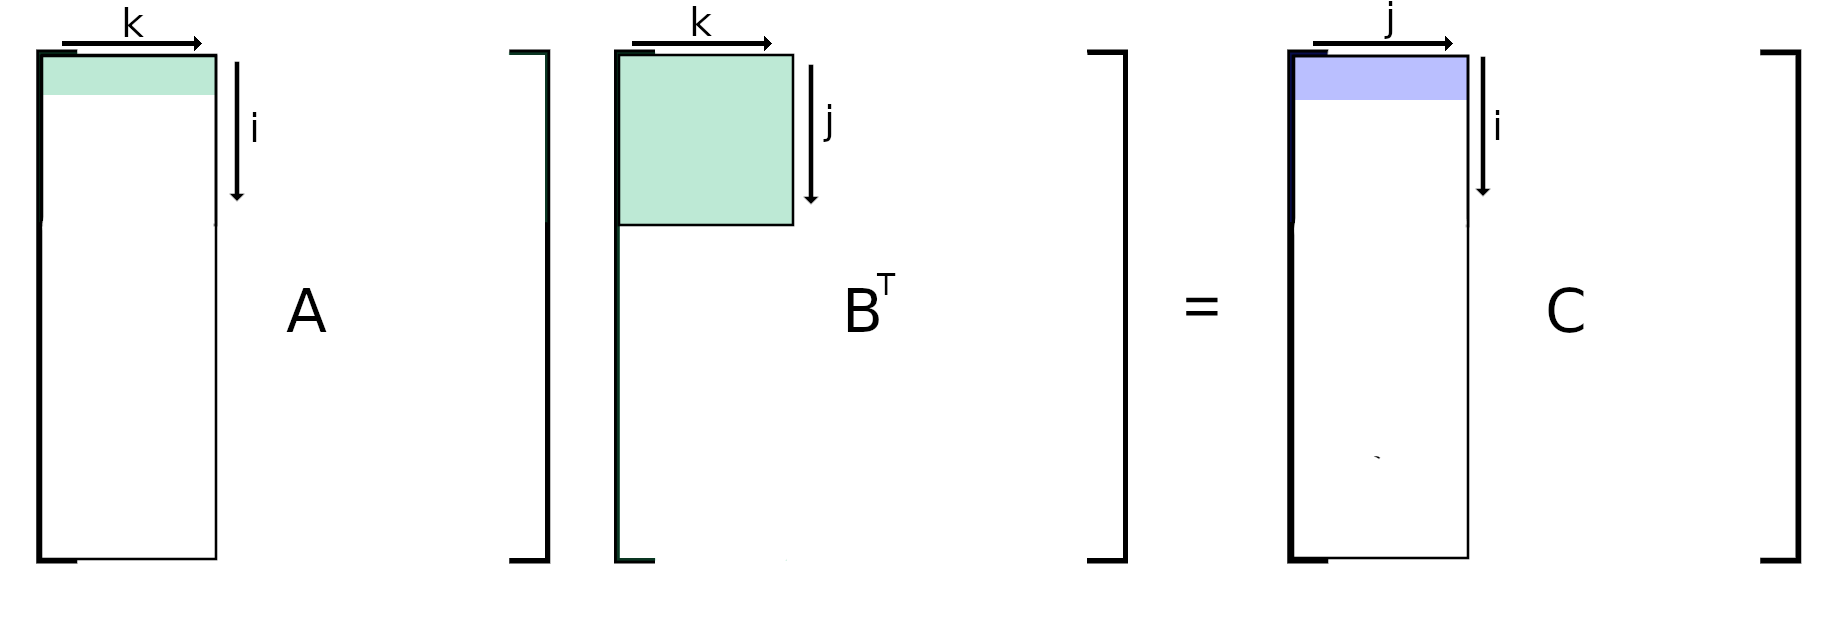
\includegraphics[width=0.7\textwidth]{images/matrix_mult_block.png}
        \caption{Dotprod with Block Optimization}
\end{figure}

After creating a working dotprod implementation with block optimization we
decided to apply the vectorization flags to the compilation and analize the
compiler output in order to check if the code was successfully vectorized. Due
to a Read after write data dependency minor tweaks had to be applied to the code
in order for it to vectorize successfully.

Finally this version of the dotprod with block optimization and vectorization
was modified to run efficiently on all cores of a multicore device making use of
OpenMP.

Due to the fact that the GPU is design to perform operations over matrices it
would be relevant to compare the performance of the optimized dotprod with the
performance of a algorithm designed to use all the SMX of a Kepler architecture.
This algorithm uses matrix blocking and GPU shared memory in order to maximize
the performance of the computation.

In this algorithm each thread calculates a position of the C matrix. Since the
shared memory is shared within a given block and contains all the values needed
to calculate a temporary block that will be added to the final block on the
matrix C, all the threads on that given block can calculate their value
accessing only the shared memory. This way the threads spend less time on the
scoreboard waiting for the memory. Due to the parallel nature of the GPU all the
blocks are being computed at the same time.

\chapter{Dotprod Benchmarking}
In order to properly benchmark the different algorithms created and compare them
we choose to collect data with PAPI and \textit{sys/time.h}. The full list of
counters available in the used system is on the Appendix \ref{A:papi_avail}. From
this list we choose to use the following PAPI counters:
\begin{verbatim}
PAPI_L1_TCM, PAPI_L2_TCM, PAPI_L3_TCM, PAPI_LD_INS, PAPI_SR_INS, PAPI_TOT_INS
\end{verbatim}

With this set of counters we can validate the theory that different algorithms
have different cache misses and memory access and also identify possible
bottlenecks related to cache misses.

To also benchmark the impact of different sizes of matrices we choose four
different matrix sizes. The smaller one fits in the L1 cache; the second
smallest fits in the L2 cache; the second largest fits in the L3 cache and
finally the biggest one requires significant access to RAM. Based on the CPU
used for benchmarking the following table was created were the formula to
calculate the max size is: \[N^2*3*sizeof(float) = cache\_size\]

\begin{table}[H]
\centering
\begin{tabular}{|l|l|l|l|l|}
\hline
           & L1 data & L2 data & L3 data  & RAM                        \\ \hline
cache size & 32768B   & 262144B  & 31457280B & \textgreater{}31457280B \\ \hline
max size   & 52      & 147     & 1619     & \textgreater{}1619         \\ \hline
used size  & 40      & 120     & 1500     & 4000                       \\ \hline
estimated FP op's & 128000  & 3456000 & 6750000000 & 1.28*10¹¹         \\ \hline
estimated RAM transfers & 19200B  & 172800B & 27000000B & 192000000B   \\ \hline
\end{tabular}
\caption{Matrix sizes used for benchmarking}
\end{table}

For the tests, the matrix A was filled with random numbers and the matrix B was
filled with ones. This way, AxB results in a matrix where all column have the
same value and BxA results in a matrix where all lines have the same value. This
property was used to assert if all the variations of the algorithm were producing
the correct results. After each test the cache was cleared to ensure all the
tests used a cold cache. To reduce the outliers, the time measurements were
performed 8 times using a K-best scheme with K=3 and a tolerance of 5\%.

\begin{table}[H]
\centering
\begin{tabular}{|l|l|l|l|l|}
\hline
            & 40x40 & 120x120 & 1500x1500 & 4000x4000 \\ \hline
i-j-k       & 66    & 1733    & 4239493   & 177553349 \\ \hline
i-j-k trans & 94    & 1698    & 3223331   & 71675215  \\ \hline
i-k-j       & 71    & 1718    & 3194044   & 61695968  \\ \hline
j-k-i       & 72    & 1744    & 8596300   & 324751067 \\ \hline
\textit{j-k-i trans} & \textit{69}    & \textit{1375}    & \textit{2273077}   &
\textit{45375529}  \\ \hline
\end{tabular}
\caption{Execution time for non-blocking sequential algorithms (time in $\mu$s)}
\end{table}

The results achieved for the \textbf{j-k-i trans} were not the expected results.
We expected that the \textbf{j-k-i trans} should be slower than \textbf{i-j-k}
due to the extra cost of transposing more matrices. However this is not what was
observed on the results. After canalizing the compiler output we realized that
the only function that vectorized was that one. Therefore, all the tables have
the line relative to this algorithm in italic.

For the 40x40 matrix the benefit for the computation that comes from transposing
the matrix is not enough to outweigh the cost of actually transposing it. For
bigger matrices the difference in times becomes even more noticeable resulting in
results one order of magnitude faster for the 4000x4000 matrix.

\begin{table}[H]
\centering
\begin{tabular}{|l|l|l|l|l|}
\hline
            & 40x40   & 120x120 & 1500x1500 & 4000x4000 \\ \hline
i-j-k       & .001321 & .000057 & .000582   & .781009   \\ \hline
i-j-k trans & .001911 & .000105 & .000308   & .084568   \\ \hline
i-k-j       & .027150 & .007252 & .000259   & .030864   \\ \hline
j-k-i       & .036501 & .008403 & .001570   & .785903   \\ \hline
\textit{j-k-i trans} & \textit{.034159} & \textit{.008555} & \textit{.000902}
                     & \textit{.053824}   \\ \hline
\end{tabular}
\caption{RAM access per total instructions (\%)}
\end{table}


\begin{table}[H]
\centering
\begin{tabular}{|l|l|l|l|l|l|}
\hline
\multicolumn{2}{|l|}{}            & 40x40 & 120x120 & 1500x1500 & 4000x4000 \\ \hline
\multirow{3}{*}{i-j-k}       & L1 & .2360 & 2,1902  & 35.5386   & 34.4700   \\ \cline{2-6}
                             & L2 & .0762 & .0237   & 2.3420    & 34.4019   \\ \cline{2-6}
                             & L3 & .0025 & .0001   & .0016     & 2.0842    \\ \hline
\multirow{3}{*}{i-j-k trans} & L1 & .1865 & 2.0801  & 2.0981    & 2.1194    \\ \cline{2-6}
                             & L2 & .0902 & .0294   & .0532     & .7009     \\ \cline{2-6}
                             & L3 & .0664 & .0196   & .0015     & .2712     \\ \hline
\multirow{3}{*}{j-k-i}       & L1 & .1411 & 1.9620  & 50.0075   & 50.1961   \\ \cline{2-6}
                             & L2 & .0873 & .0273   & 9.6299    & 50.1126   \\ \cline{2-6}
                             & L3 & .0709 & .0173   & .0031     & 1.5741    \\ \hline
\multirow{3}{*}{\textit{j-k-i trans}} & \textit{L1} & \textit{.6037} & \textit{7.9182}  & \textit{8.4272}    & \textit{8.5532}    \\ \cline{2-6}
                                      & \textit{L2} & \textit{.3874} & \textit{.1204}   & \textit{.2507}     & \textit{6.4841}    \\ \cline{2-6}
                                      & \textit{L3} & \textit{.3270} & \textit{.0831}   & \textit{.0087}     & \textit{2.9880}    \\ \hline
\end{tabular}
\caption{Global miss rate for algoritms that benefited from transposing}
\end{table}

Analysing this table we can confirm the theory that transposing the matrix
in order to access it line by line has, in fact, the result of reducing cache
misses. The outlier in this case is the \textbf{j-k-i trans} that actually
increased the global miss rate. After carefully analysing the results we
realized that the cache misses for a given cache remained mostly the same
between \textbf{j-k-i} and \textbf{j-k-i trans}, what greatly decreased was the
number of load and store instructions. Since the formula used for calculating
the global miss rate divides the number of cache misses for a given cache level
by the total number of memory access, reducing the number of memory access
increases the global miss rate.

\begin{table}[H]
\centering
\begin{tabular}{|l|l|l|l|}
\hline
          & i-j-k trans & i-j-k trans + block & speedup \\ \hline
4000x4000 & 71675215    & 64385275            & 1.1132  \\ \hline
\end{tabular}
\caption{Time comparison of block optimisation (time in $\mu$)}
\end{table}

\begin{table}[H]
\centering
\begin{tabular}{|l|l|l|l|}
\hline
        & i-j-k trans & i-j-k trans + block + vec & speedup \\ \hline
40x40   & 94          & 71                        & 1.3239  \\ \hline
120x120 & 1698        & 1523                      & 1.1149  \\ \hline
\end{tabular}
\caption{Time comparison of block optimization with vectorization (time in
$\mu$)}
\end{table}

\begin{table}[H]
\centering
\begin{tabular}{|l|l|l|l|}
\hline
          & i-j-k trans & i-j-k trans + block + vec + OpenMP & speedup \\ \hline
4000x4000 & 71675215    & 2407551                            & 29.7710 \\ \hline
\end{tabular}
\caption{Time comparison of block optimization with vectorization and OpenMP (time in
$\mu$)}
\end{table}

The blocking of the algorithm gratly reduces the time of the algorithm. Simply
adding blocking we achieved a speedup of 1.1132. Adding vectorization we were
able to achieve a speedup of 1.3239 for the smallest matrix. Finnaly, adding
parallelism with OpenMP to the vectorized code yielded a speedup of 29.7710.

\begin{table}[H]
\centering
\begin{tabular}{|l|l|l|l|l|}
\hline
        & Computation & Host to Device & Device to Host & Total \\ \hline
120x120 & 195         & 33             & 9              & 640   \\ \hline
512x512 & 1390        & 524            & 154            & 4206  \\ \hline
\end{tabular}
\caption{Analysis of CUDA times (time in $\mu$s)}
\end{table}

\begin{table}[H]
\centering
\begin{tabular}{|l|l|l|}
\hline
                          & 120x120 & Speedup \\ \hline
CUDA                      & 640     & 1.0000  \\ \hline
i-j-k trans + block + vec & 1523    & 2.3796  \\ \hline
i-j-k trans               & 1698    & 2.6531  \\ \hline
\end{tabular}
\caption{Time comparison of CUDA (time in $\mu$s)}
\end{table}


\chapter{Conclusions}

After the analysis of the results collected during the elaboration of this
report, we can conclude that memory access optimizations can greatly
impact an algorithm performance, reducing cache misses, therefore, reducing the
data wait time of the processor.
We can also conclude that GPU processing can be a lot faster to process
matrices than a CPU, due to its inherently parallel architecture.

\appendix

\chapter{Roofline of the 662 node}
\begin{figure}[H]
    \centering
        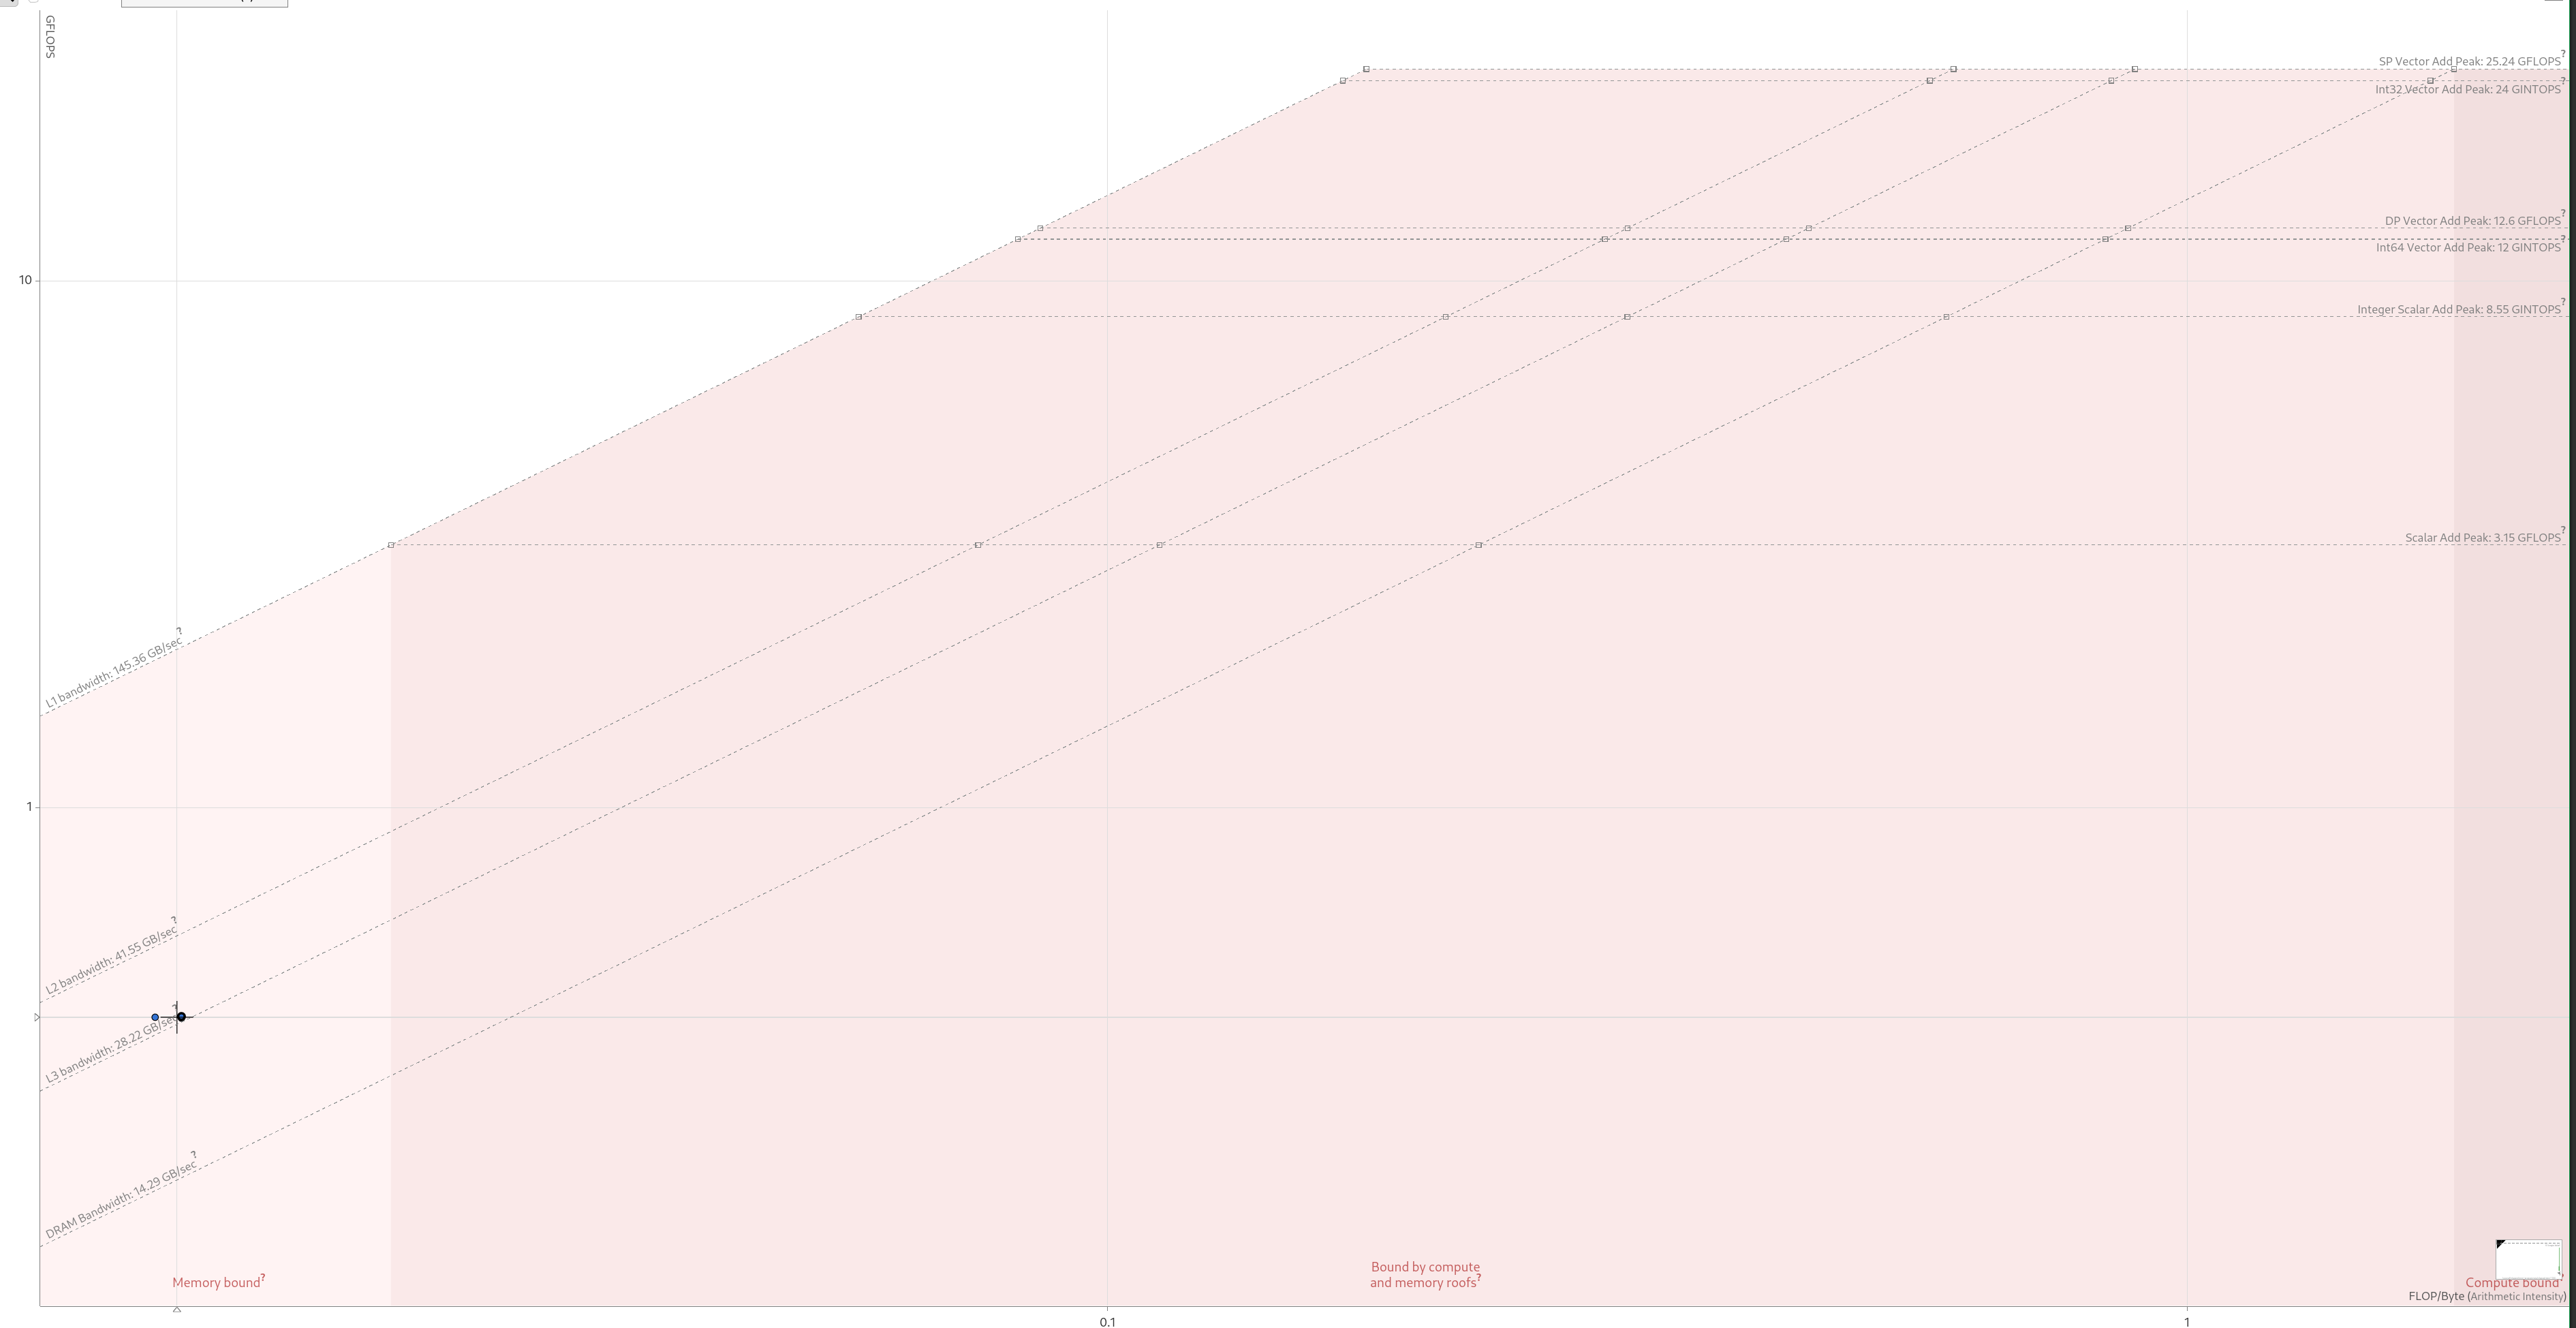
\includegraphics[width=\textwidth]{images/roofline_cluster.png}
        \caption{roofline on the 662 node}
\end{figure}

\chapter{Available papi counters}\label{A:papi_avail}
\verbatiminput{papi_avail_-a.txt}

\end{document}
